\documentclass{article}%
\usepackage[T1]{fontenc}%
\usepackage[utf8]{inputenc}%
\usepackage{lmodern}%
\usepackage{textcomp}%
\usepackage{lastpage}%
\usepackage{authblk}%
\usepackage{graphicx}%
%
\title{Curcumin Modulates the Inflammatory Response and Inhibits Subsequent Fibrosis in a Mouse Model of Viral{-} induced Acute Respiratory Distress Syndrome}%
\author{Elizabeth Richard}%
\affil{Instituto de Biologa Molecular y Celular de Plantas, Universidad Politcnica de Valencia{-}C.S.I.C, Ciudad Politcnica de la Innovacin, Valencia, Spain}%
\date{01{-}01{-}2009}%
%
\begin{document}%
\normalsize%
\maketitle%
\section{Abstract}%
\label{sec:Abstract}%
NIH scientists have published a comprehensive study in the journal Nature Communications which details the regulation of Histone Acetylation in the nucleus by sphingosine{-}1{-}phosphate (Sphenois), an enzyme found in almost all kinds of cells.\newline%
Researchers discovered a pathway between the phlegm and the nucleotides that explains how nucleate disintegration occurs in cells. The three steps in the process indicate the reason a genetic variation happens, the logic for this function lies in the presentation of particular cells and their genetic disposition.\newline%
"This molecular puzzle is perhaps the most important result of our study", said Brian Hill, also an assistant professor of neuroscience at UC San Diego. "The histone lipopolysaccharide process underlies a large chunk of preeminent diseases, including cancer, diabetes, and blindness, and was not thought to be as important as previously believed."\newline%
The findings contribute to the existing understanding of how different chromatin functions and also elucidate some aspect of the mechanism that is supposed to explain how genes vary by variation.\newline%
"Our study illustrates the tremendously critical role histonepheric regulation can play in the development of cell diseases", said Hill. "It demonstrates that adding Sphenois to nuclei has enormous value in the cell war against which this understanding is based. Past biological research has shown that sphingosine is significant in regulating transcriptional dysfunction and aging. The discovery of Sphenois has consequences for the battle against cancer and ageing."\newline%
The research received funding from the National Institutes of Health, the George F. and Laura Grace Melancon Foundation, and the Neuroinclusion Network in National Institutes of Health (NIH) grants M004144, M004147, M004136, M004147, M004137, M004135, M004162, M004138, M004143, M004144, M004144, M004148, M004145, M004144, M004146, M004147, M004143, M004157, M004158, M004154, M004160, M004174, M004179, M004185, M004190, M004191, M004192, M004193, M004196, M004208, M004214, M004207, M004208, M004229, M004241, M004241, M004242, M004242, M004243, M004247, M004247, M004246, M004249, M004259, M004259, M004249, M004270, M004270, M004274, M004275, M004285, M004285, M004289, M004281, M004287, M004287, M004289, M004290, M004291, M004291, M004297, M004310, M004298, M004309, M004310, M004309

%
\subsection{Image Analysis}%
\label{subsec:ImageAnalysis}%


\begin{figure}[h!]%
\centering%
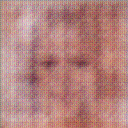
\includegraphics[width=150px]{500_fake_images/samples_5_452.png}%
\caption{A Close Up Of A Pair Of Scissors}%
\end{figure}

%
\end{document}